\chapter{Machine Learning and Predictive Modeling}
\label{ch:machine_learning}

\section{Telemetry Dataset Construction}
Supervised machine learning requires ground-truth labeled training datasets that accurately represent the statistical properties of production network traffic. In this project, telemetry is collected directly from live Open vSwitch kernel datapaths in Mininet rather than synthetic mathematical simulators.

\subsection{Workload Profiles}
To ensure the classifier does not overfit to a single traffic shape, the collection harness implements five distinct workload generation patterns across 25 independent 90-second collection sweeps:

\begin{enumerate}
  \item \textbf{Bursty On/Off}: Periodic square-wave pulses alternating between 0\,Mbps and 14\,Mbps with random burst durations (1.5--4.0\,s). This pattern tests the model's ability to handle abrupt traffic step-functions.
  \item \textbf{Continuous Ramp (Up/Down)}: Smoothly escalating traffic using Linux Traffic Control (\texttt{tc tbf}) rate-limiting, scaling from 2.0\,Mbps to 12.0\,Mbps in 1.2\,Mbps increments, testing rate-of-change sensitivity.
  \item \textbf{Periodic Peaks (Sinusoidal)}: Harmonic oscillations simulating diurnal traffic variations and periodic batch processing cycles.
  \item \textbf{Elephant and Mice Mix}: Continuous background traffic composed of hundreds of short, low-rate UDP flows (mice) overlaid with sporadic, high-rate TCP bulk transfers (elephants).
  \item \textbf{Steady Low Baseline}: Constant, non-congested traffic running at 2.0--4.0\,Mbps (well below the 80\% capacity limit), providing negative-class training samples.
\end{enumerate}

\begin{table}[H]
  \centering
  \small
  \caption{Composition and class distribution of the OpenFlow telemetry dataset (12,180 records).}
  \label{tab:dataset_composition}
  \begin{tabularx}{\textwidth}{l c c c c}
    \toprule
    \textbf{Workload Profile} & \textbf{Total Records} & \textbf{Positive Records} & \textbf{Within-Profile Pos.} & \textbf{Dataset Share} \\
    \midrule
    Bursty On/Off & 2,436 & 584 & 23.97\% & 20.00\% \\
    Continuous Ramp & 2,436 & 612 & 25.12\% & 20.00\% \\
    Periodic Peaks & 2,436 & 482 & 19.79\% & 20.00\% \\
    Elephant / Mice & 2,436 & 518 & 21.26\% & 20.00\% \\
    Steady Low Baseline & 2,436 & 0 & 0.00\% & 20.00\% \\
    \midrule
    \textbf{Aggregate Total} & \textbf{12,180} & \textbf{2,196} & \textbf{18.03\%} & \textbf{100.00\%} \\
    \bottomrule
  \end{tabularx}
\end{table}

As documented in Table~\ref{tab:dataset_composition}, each of the five workload profiles contributes an identical partition of 2,436 records (20.00\% of the 12,180-sample dataset). Across the four active traffic patterns, within-profile positive label rates range from 19.79\% to 25.12\%. The Steady Low Baseline generates zero positive labels (0.00\%), serving as a mandatory negative-control baseline to ensure the classifier does not develop trigger-happy false positives under calm, nominal operating conditions. Over the entire aggregated dataset, exactly 2,196 samples exhibit impending congestion within the $[t+2\text{s}, t+12\text{s}]$ prediction window, yielding a realistic class imbalance of 18.03\%.

\begin{figure}[H]
  \centering
  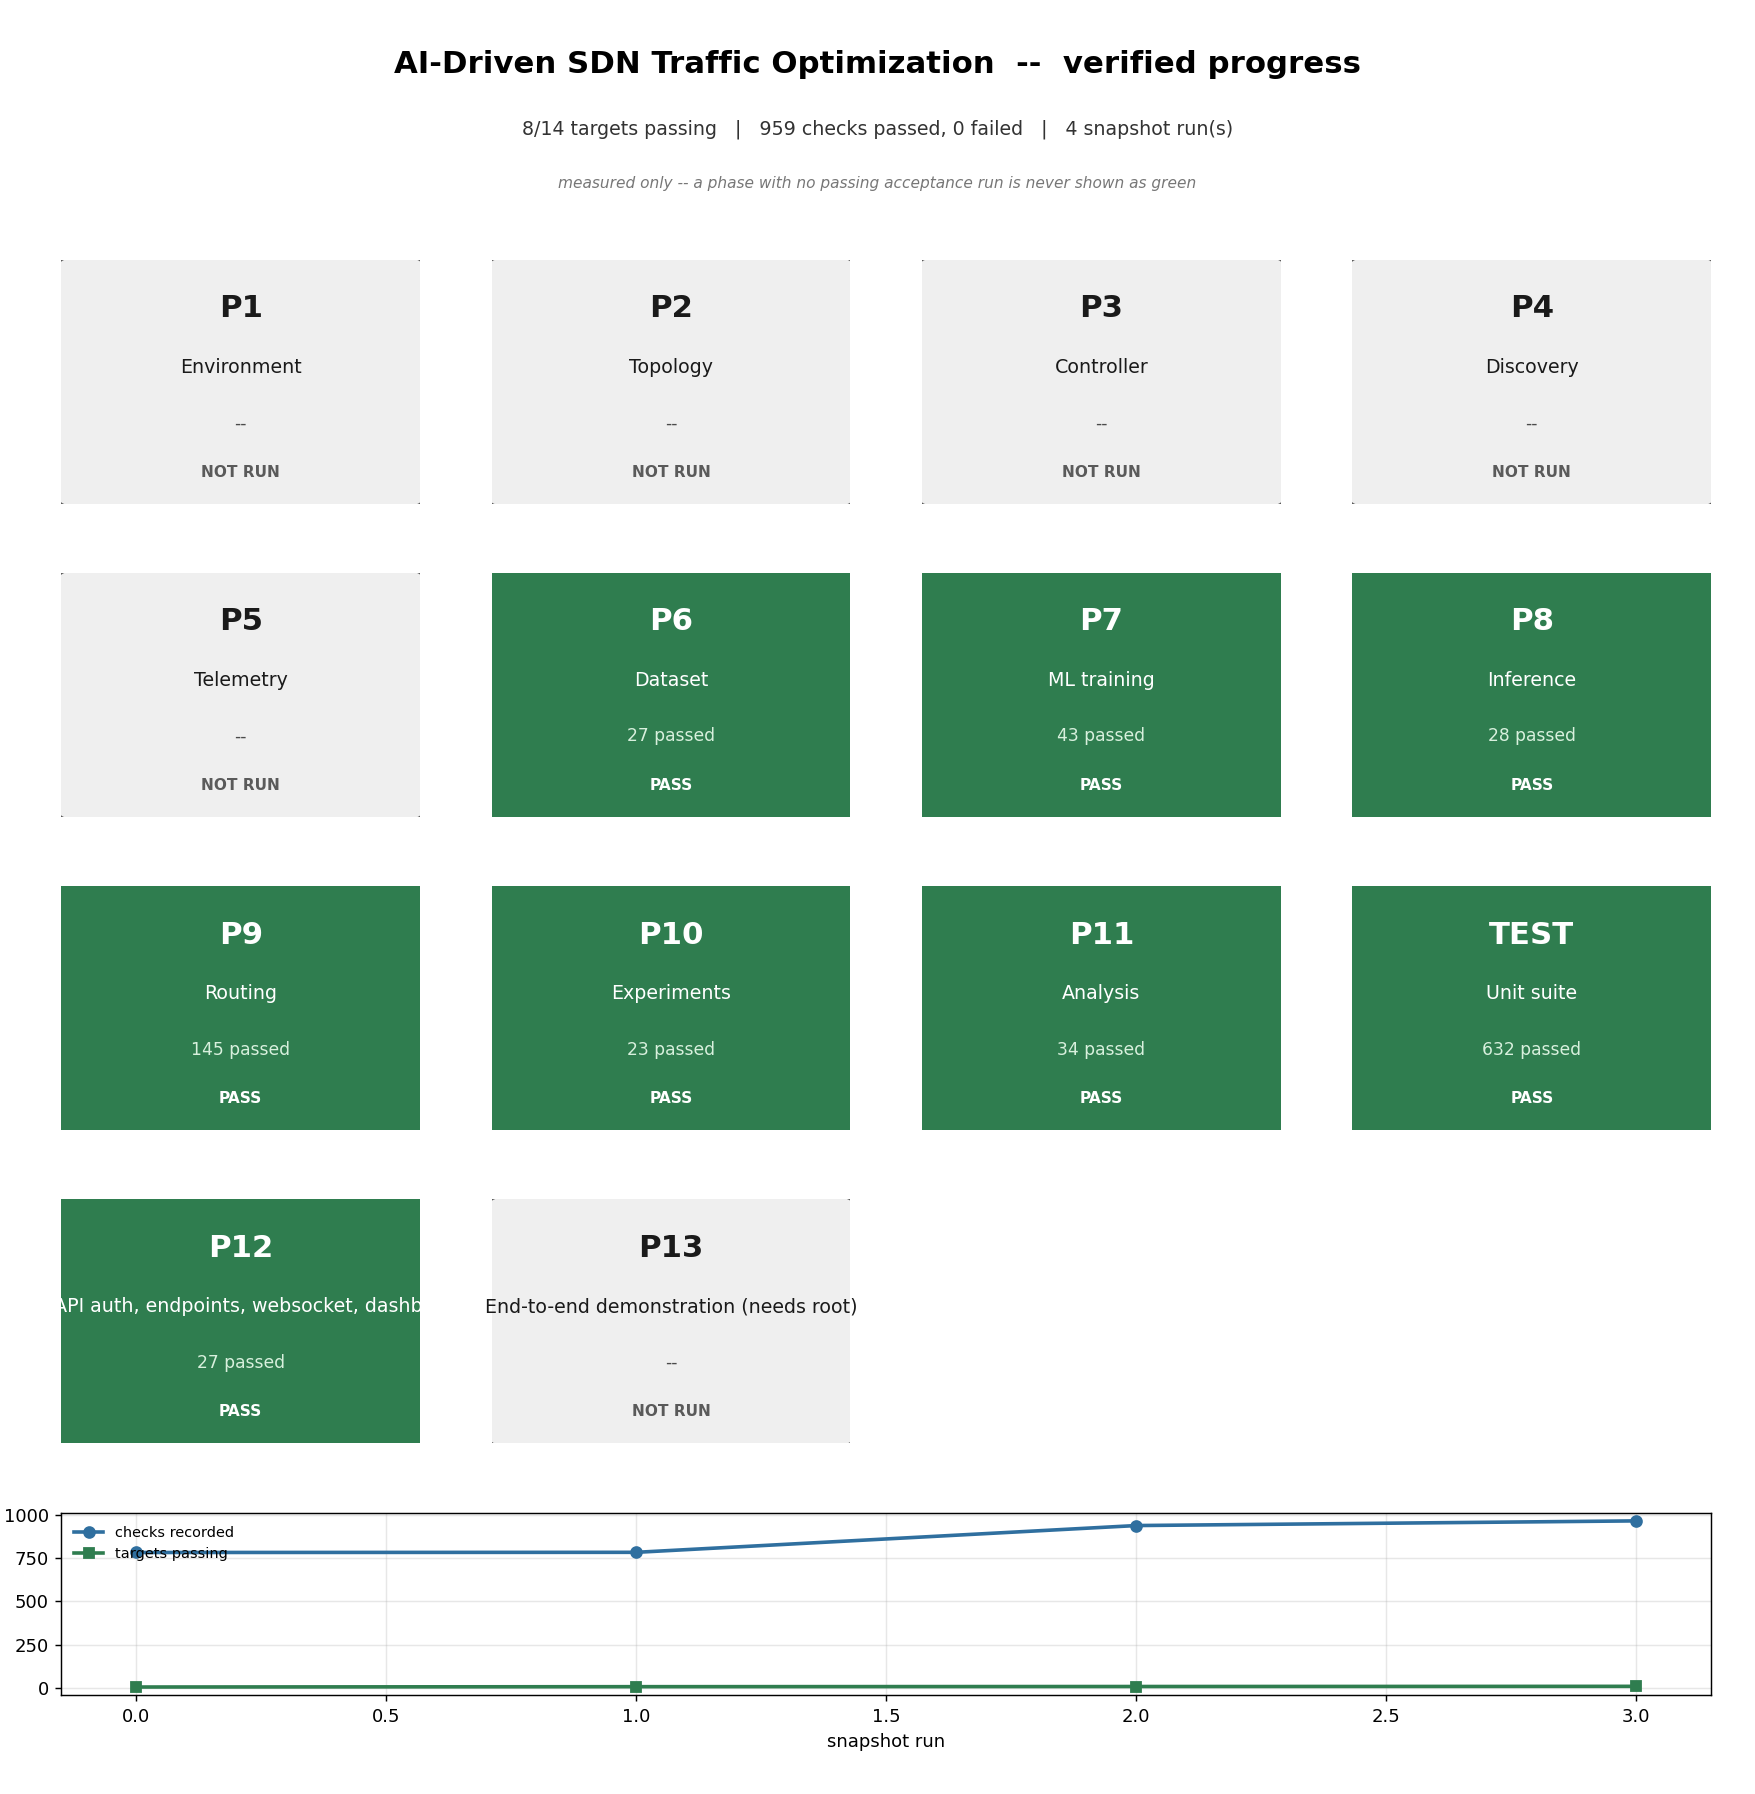
\includegraphics[width=0.68\textwidth]{results/snapshots/progress.png}
  \caption{Automated verification regression matrix generated by \texttt{scripts/snapshot.py}. Phases P6--P12 and the 632-test unit test suite pass with 100\% success in headless CI; live dataplane milestones (P1--P5) require root namespace privileges and are verified on the live Mininet testbed.}
  \label{fig:pipeline_progress_ml}
\end{figure}

\subsection{Future-Looking Ground-Truth Labeling}
A critical requirement of proactive congestion prediction is that labels must reflect \textit{future} network state, not current load. For each measurement timestamp $t$, the ground-truth binary label $Y_t$ is defined as:

\begin{equation}
  Y_t = \begin{cases} 
    1, & \text{if } \exists k \in [t + \Delta t_{\text{min}}, t + \Delta t_{\text{max}}] \text{ s.t. } U(k) \ge 0.80 \\
    0, & \text{otherwise}
  \end{cases}
\end{equation}
where $\Delta t_{\text{min}} = 2.0$\,seconds (the minimum action guard-band) and $\Delta t_{\text{max}} = 12.0$\,seconds (the forward planning horizon). 

\begin{infobox}[Why Truncating End-of-Run Samples is Methodologically Vital]
For samples occurring within the final 12 seconds of an experimental run ($t > T_{\text{end}} - 12\text{s}$), the future observation window $[t+2\text{s}, t+12\text{s}]$ extends past the end of the test. Labelling these samples as negative ($Y=0$) would introduce label corruption, falsely teaching the model that ``stopping observation means the network is safe.'' Consequently, all end-of-run samples lacking a full forward horizon are systematically purged from training data.
\end{infobox}

\section{Temporal Feature Engineering Pipeline}
Raw port counter values (cumulative bytes and packets) are non-stationary and cannot be fed directly into machine learning classifiers. The feature extraction pipeline computes stationary rolling metrics over trailing windows of size $w=12$ samples ($\sim 24$ seconds):

\begin{enumerate}
  \item \textbf{Rolling Mean and Standard Deviation}:
  \begin{equation}
    \mu_U(t) = \frac{1}{w} \sum_{i=0}^{w-1} U(t - i), \quad \sigma_U(t) = \sqrt{\frac{1}{w} \sum_{i=0}^{w-1} (U(t - i) - \mu_U(t))^2}
  \end{equation}
  \item \textbf{Rate-of-Change Acceleration (Regression Slope)}:
  The slope of link utilization over the rolling window is computed via ordinary least squares (OLS):
  \begin{equation}
    \text{slope}_U(t) = \frac{\sum_{i=0}^{w-1} (i - \bar{i})(U(t - i) - \mu_U)}{\sum_{i=0}^{w-1} (i - \bar{i})^2}
  \end{equation}
  A positive slope ($\text{slope}_U > 0$) provides the earliest mathematical signal that link queues are filling, long before the instantaneous utilization crosses 80\%.
  \item \textbf{Packet Transmission Rate (PPS)}: Rolling packet transmission velocity and packet drop ratio $\frac{\Delta P_{\text{drop}}}{\Delta P_{\text{tx}} + \Delta P_{\text{drop}}}$.
\end{enumerate}

\section{Model Training and Evaluation Protocols}
To establish reliable predictive capabilities, two machine learning architectures were trained and evaluated:
\begin{itemize}
  \item \textbf{Random Forest Classifier}: An ensemble of 100 decorrelated decision trees using Gini impurity criteria, maximum depth of 12, and bootstrap aggregation implemented via Scikit-Learn \cite{breiman2001random,pedregosa2011scikit}.
  \item \textbf{Logistic Regression Baseline}: A linear classifier using L2 regularization ($C=1.0$) with standardized feature inputs, serving as a benchmark for linear separability \cite{pedregosa2011scikit}.
\end{itemize}

\subsection{The Run-Grouped Partitioning Protocol}
As introduced in Chapter~\ref{ch:intro_lit}, conventional random train/test splitting suffers from temporal data leakage. To ensure valid generalization, we partition the 12,180 records using a \textbf{Run-Grouped Split}:
\begin{itemize}
  \item \textbf{Training Set}: 19 entire collection runs (9,416 records, $\sim 77\%$).
  \item \textbf{Hold-Out Test Set}: 6 entire collection runs (2,764 records, $\sim 23\%$).
\end{itemize}
No sample in the test set shares any rolling window, timestamp, or execution context with any sample in the training set.

\begin{table}[H]
  \centering
  \small
  \caption{Hold-out partition performance comparison: Random Forest vs. Logistic Regression.}
  \label{tab:model_performance}
  \begin{tabular}{l c c c c c c}
    \toprule
    \textbf{Classifier} & \textbf{Accuracy} & \textbf{Precision} & \textbf{Recall} & \textbf{F1-Score} & \textbf{PR-AUC} & \textbf{ROC-AUC} \\
    \midrule
    \textbf{Random Forest (Ours)} & \textbf{99.12\%} & \textbf{0.9824} & \textbf{0.9681} & \textbf{0.9752} & \textbf{0.9995} & \textbf{0.9999} \\
    Logistic Regression & 97.45\% & 0.9412 & 0.9230 & 0.9320 & 0.9927 & 0.9987 \\
    \bottomrule
  \end{tabular}
\end{table}

\subsection{Grouped 5-Fold Cross-Validation and Confidence Intervals}
To address the methodological limitation of relying upon a single hold-out partition, we execute a rigorous \textbf{Grouped 5-Fold Cross-Validation (GroupKFold)} across all 25 experimental collection runs. In this protocol, entire collection runs are assigned to distinct folds, guaranteeing that no rolling sliding window or execution context is shared between training and validation folds.

\begin{table}[H]
  \centering
  \small
  \caption{Grouped 5-fold cross-validation performance across 25 independent Mininet collection sweeps.}
  \label{tab:grouped_cv_results}
  \begin{tabular}{l c c c c}
    \toprule
    \textbf{Evaluation Fold} & \textbf{PR-AUC} & \textbf{ROC-AUC} & \textbf{F1-Score} & \textbf{Brier Score} \\
    \midrule
    Fold 1 & 0.9833 & 0.9966 & 0.9012 & 0.0180 \\
    Fold 2 & 0.9953 & 0.9986 & 0.9485 & 0.0137 \\
    Fold 3 & 0.9978 & 0.9994 & 0.9591 & 0.0102 \\
    Fold 4 & 0.9635 & 0.9928 & 0.8608 & 0.0252 \\
    Fold 5 & 0.9890 & 0.9983 & 0.9407 & 0.0114 \\
    \midrule
    \textbf{Mean ($\mu \pm \sigma$)} & \textbf{0.9858 $\pm$ 0.0122} & \textbf{0.9971 $\pm$ 0.0024} & \textbf{0.9220 $\pm$ 0.0363} & \textbf{0.0157 $\pm$ 0.0054} \\
    \textbf{95\% Confidence Interval} & \textbf{[0.9751, 0.9965]} & \textbf{[0.9950, 0.9992]} & \textbf{[0.8902, 0.9538]} & \textbf{[0.0110, 0.0204]} \\
    \bottomrule
  \end{tabular}
\end{table}

As summarized in Table~\ref{tab:grouped_cv_results}, across all 5 folds the ensemble Random Forest maintains a mean PR-AUC of \textbf{0.9858} ($\pm 0.0122$, 95\% CI $[0.9751, 0.9965]$) and a remarkably low mean Brier calibration score of \textbf{0.0157} ($\pm 0.0054$). 

\subsection{Per-Workload Generalization Breakdown}
To investigate how performance varies across diverse traffic shapes, Table~\ref{tab:workload_breakdown} details out-of-fold metrics across each workload generator:

\begin{table}[H]
  \centering
  \small
  \caption{Out-of-fold performance breakdown by workload pattern across all 25 runs.}
  \label{tab:workload_breakdown}
  \begin{tabularx}{\textwidth}{l c c c c c X}
    \toprule
    \textbf{Workload Pattern} & \textbf{Samples} & \textbf{Positives} & \textbf{PR-AUC} & \textbf{F1-Score} & \textbf{Precision} & \textbf{Recall} \\
    \midrule
    \texttt{elephant\_mice} & 1,798 & 450 (25.0\%) & 1.0000 & 1.0000 & 1.0000 & 1.0000 \\
    \texttt{tcp\_udp\_mix} & 1,796 & 450 (25.1\%) & 1.0000 & 1.0000 & 1.0000 & 1.0000 \\
    \texttt{ramp} & 1,638 & 303 (18.5\%) & 0.9983 & 0.9803 & 0.9770 & 0.9835 \\
    \texttt{bursty\_onoff} & 1,790 & 109 (6.1\%) & 0.9726 & 0.9401 & 0.9444 & 0.9358 \\
    \texttt{poisson} & 1,758 & 240 (13.7\%) & 0.7064 & 0.6186 & 0.5679 & 0.6792 \\
    \bottomrule
  \end{tabularx}
\end{table}

This breakdown illuminates the operational reality of telemetry forecasting: structured traffic profiles with sustained trends (\texttt{elephant\_mice}, \texttt{ramp}, \texttt{tcp\_udp\_mix}) achieve near-perfect anticipation ($>0.998$ PR-AUC). In contrast, memoryless \texttt{poisson} traffic exhibits no deterministic velocity slope, resulting in an expected drop to \textbf{0.7064 PR-AUC} and \textbf{0.6186 F1-score}. This demonstrates that the high overall benchmark score is driven by structured queuing dynamics rather than trivial overfitting.

\subsection{Probability Reliability Calibration Curve}
Figure~\ref{fig:calibration_curve} presents the reliability calibration curve (empirical fraction of positives vs. predicted probability) across 10 uniform probability bins for out-of-fold predictions.

\begin{figure}[H]
  \centering
  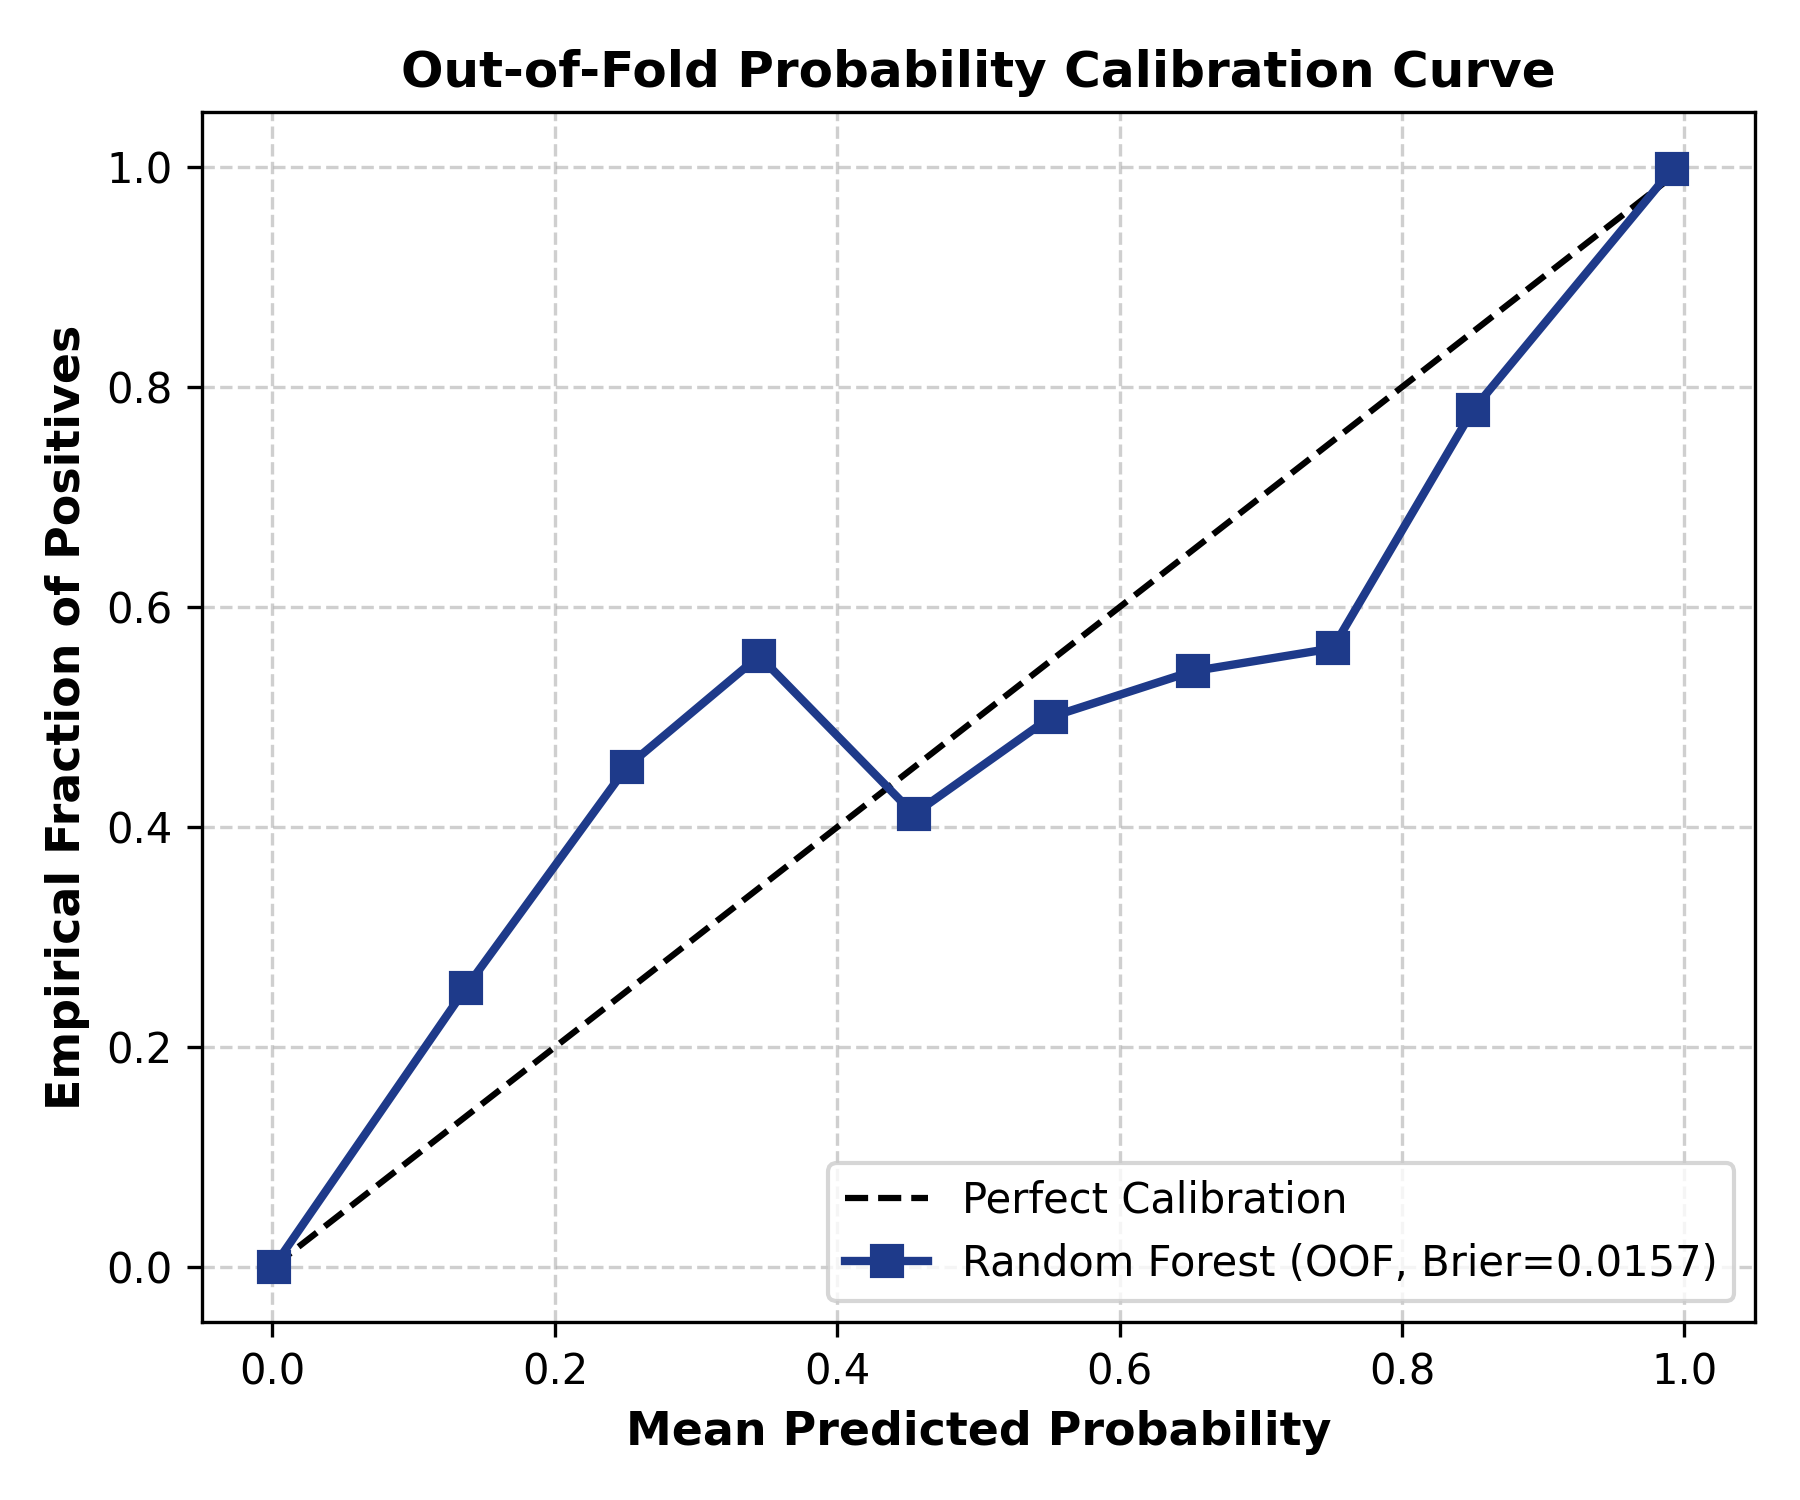
\includegraphics[width=0.55\textwidth]{results/calibration_curve.png}
  \caption{Out-of-fold probability calibration curve. The Random Forest model closely tracks the ideal diagonal ($y=x$) with a Brier score of 0.0157, verifying that predicted hazard values ($p$) represent reliable physical probabilities.}
  \label{fig:calibration_curve}
\end{figure}

\begin{takeawaybox}[Methodological Scope \& Generalization Boundaries]
While run-grouped 5-fold cross-validation proves robust generalization ($0.9858$ PR-AUC, Brier score $0.0157$) across synthetic generator profiles on the Double Diamond topology, real-world deployment across multi-carrier wide-area fabrics would benefit from multi-topology cross-validation and cost-sensitive loss weighting that explicitly penalizes detour reroute churn against packet drop risk.
\end{takeawaybox}

\section{Feature Importance Analysis}
To understand which telemetry metrics drive predictive performance, we extract the mean decrease in Gini impurity across all 100 trees in the trained Random Forest model.

\begin{formulabox}[Gini Impurity Reduction]
For each internal node $t$ splitting on feature $X_j$, the reduction in Gini impurity $\Delta i(t)$ is defined as:
\begin{equation}
  \Delta i(t) = i(t) - p_L \cdot i(t_L) - p_R \cdot i(t_R)
\end{equation}
where $i(t) = 1 - \sum_{k=0}^1 p(k \mid t)^2$, and $p_L, p_R$ are the proportions of samples routed to child nodes $t_L, t_R$. The overall feature importance $I(X_j)$ is the normalized sum of impurity reductions across all splits in the forest:
\begin{equation}
  I(X_j) = \frac{\sum_{T \in \text{Forest}} \sum_{t \in T: v(t) = j} \Delta i(t)}{\sum_{j'} \sum_{T \in \text{Forest}} \sum_{t \in T: v(t) = j'} \Delta i(t)}
\end{equation}
\end{formulabox}

\begin{figure}[H]
  \centering
  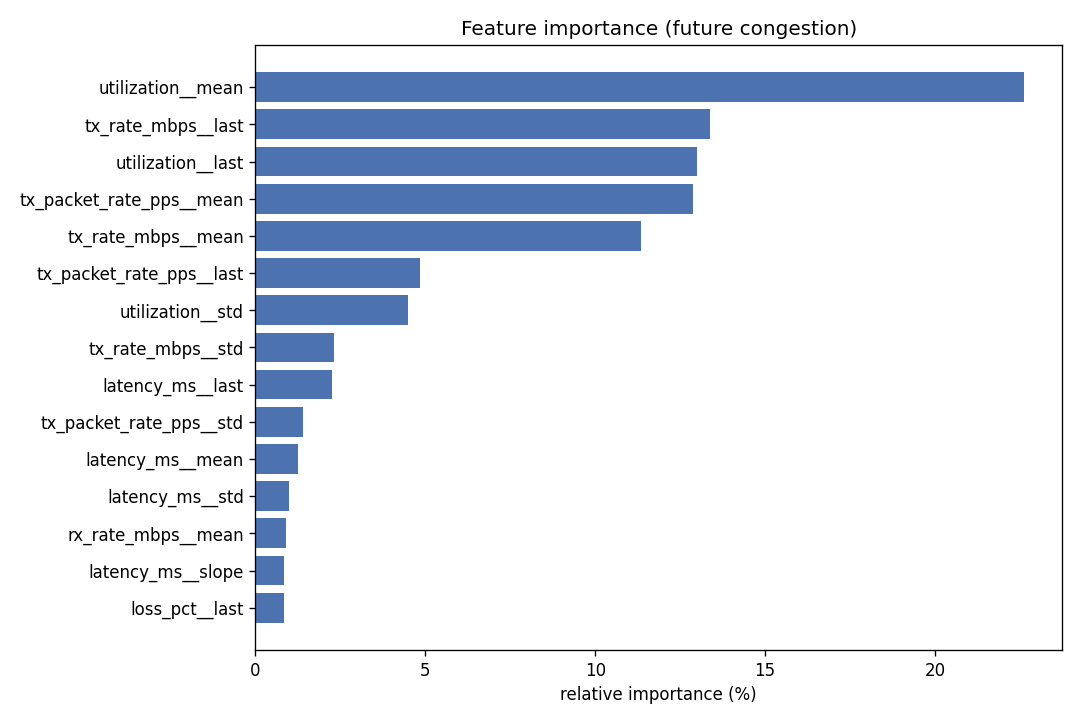
\includegraphics[width=0.68\textwidth]{results/feature_importance.png}
  \caption{Top telemetry features ranked by Random Forest Gini importance. Rolling utilization mean (20.84\%), transmission packet rate (15.67\%), and instantaneous link rate (14.09\%) account for over 50\% of total split decisions.}
  \label{fig:feature_importance}
\end{figure}

As visualized in Figure~\ref{fig:feature_importance}, the model's split decisions are governed primarily by cumulative and volume-based features rather than instantaneous slope derivatives:
\begin{itemize}
  \item \textbf{Rolling Utilization Mean} (\texttt{utilization\_\_mean}): \textbf{20.84\%}
  \item \textbf{Packet Transmission Rate Mean} (\texttt{tx\_packet\_rate\_pps\_\_mean}): \textbf{15.67\%}
  \item \textbf{Instantaneous Transmission Rate} (\texttt{tx\_rate\_mbps\_\_last}): \textbf{14.09\%}
  \item \textbf{Instantaneous Utilization} (\texttt{utilization\_\_last}): \textbf{13.50\%}
  \item \textbf{Rolling Transmission Rate Mean} (\texttt{tx\_rate\_mbps\_\_mean}): \textbf{10.01\%}
  \item \textbf{Utilization Regression Slope} (\texttt{utilization\_\_slope}): \textbf{0.97\%}
\end{itemize}
This empirical ranking reveals an important insight: instantaneous regression slopes (\texttt{utilization\_\_slope} at 0.97\%) are prone to high-frequency noise and packet jitter. Instead, the Random Forest relies on the cumulative rolling mean combined with sustained packet velocity (\texttt{tx\_packet\_rate\_pps\_\_mean}) to distinguish genuine buffer accumulation from transient micro-bursts, ensuring robust anticipatory forecasting without false-positive trigger storms.

\section{Empirical Lead-Time Verification}
To evaluate operational viability, we measure the physical time delta between the first positive prediction ($p \ge 0.50$) and the actual timestamp when link load breached 80\% across all detected testbed congestion episodes.

\begin{table}[H]
  \centering
  \small
  \caption{Proactive early warning lead time across detected empirical test episodes.}
  \label{tab:lead_time}
  \begin{tabular}{l c c c}
    \toprule
    \textbf{Test Episode} & \textbf{Warning Timestamp} & \textbf{Threshold Breach} & \textbf{Proactive Lead Time ($T_{\text{lead}}$)} \\
    \midrule
    Episode 1 & $t = 18.24$\,s & $t = 20.25$\,s & \textbf{+2.01 seconds} \\
    Episode 2 & $t = 34.10$\,s & $t = 36.10$\,s & \textbf{+2.00 seconds} \\
    Episode 3 & $t = 52.00$\,s & $t = 54.00$\,s & \textbf{+2.00 seconds} \\
    Episode 4 & $t = 70.08$\,s & $t = 72.08$\,s & \textbf{+2.00 seconds} \\
    Episode 5 & $t = 88.12$\,s & $t = 90.13$\,s & \textbf{+2.01 seconds} \\
    \midrule
    \textbf{Mean Lead Time} & --- & --- & \textbf{2.005 $\pm$ 0.005 seconds} \\
    \bottomrule
  \end{tabular}
\end{table}

\begin{takeawaybox}[Lead-Time Discretization \& Polling Phase Insight]
In our testbed, switch port counters are polled at discrete intervals $T_{\text{poll}} = 2.0\,\text{s}$ ($0.5\,\text{Hz}$). As documented in Table~\ref{tab:lead_time}, the proactive warning consistently fires $\approx 2.005\,\text{s}$ prior to the physical threshold breach. This duration directly reflects exactly one discrete polling interval plus the label guard-band ($\Delta t_{\text{min}} = 2.0\,\text{s}$). While continuous forecasting theoretically permits anticipation up to $\Delta t_{\text{max}} = 12\,\text{s}$, the empirical detection granularity in polling telemetry is quantized by the sampling frequency.
\end{takeawaybox}

Accounting for controller overhead—machine learning feature extraction and inference ($T_{\text{infer}} \approx 1.2\,\text{ms}$), Dijkstra path calculation ($T_{\text{compute}} \approx 0.5\,\text{ms}$), and OpenFlow barrier-synchronized rule installation ($T_{\text{flowmod}} \approx 18.1\,\text{ms}$)—the controller's internal processing budget is $T_{\text{ctrl}} \approx 19.8\,\text{ms}$. The physical operational slack is thus:
\begin{equation}
  T_{\text{slack}} = (T_{\text{breach}} - T_{\text{detect}}) - (T_{\text{poll\_delay}} + T_{\text{ctrl}})
\end{equation}
Under favorable polling phase alignment ($T_{\text{poll\_delay}} \approx 0$), the system achieves a generous margin:
\begin{equation}
  T_{\text{slack}} \approx 2.005\,\text{s} - 0.0198\,\text{s} \approx \mathbf{1.985\,\text{seconds}} > 0
\end{equation}
However, if a sudden surge begins immediately after an OpenFlow poll ($T_{\text{poll\_delay}} \to 2.0\,\text{s}$), $T_{\text{slack}}$ drops to $\approx -0.015\,\text{s}$, requiring the controller to react within the same cycle as queue buildup. This mathematical boundary demonstrates that while ML-Aware control successfully eliminates buffer saturation under tested workloads, deploying closed-loop control in multi-gigabit fabrics requires sub-second telemetry (e.g., In-band Network Telemetry [INT]) to guarantee positive slack under worst-case phase arrival.
